\documentclass[10pt]{extarticle}
\usepackage[paperwidth=7.07in,paperheight=9.43in,margin=0.95in]{geometry}
\usepackage{fontspec}
\setmainfont{Latin Modern Roman}
\setmonofont{Menlo}[Scale=0.85]
\usepackage{amsmath,amssymb}
\usepackage{booktabs,tabularx}
\usepackage{enumitem}
\usepackage{microtype}
\usepackage{tikz}
\usetikzlibrary{arrows.meta,positioning,calc,fit}
\tikzset{>=Stealth}
\tikzset{every picture/.append style={line width=0.6pt,font=\footnotesize}}
\usepackage[hidelinks]{hyperref}
\usepackage{parskip}
\usepackage{ragged2e}
\linespread{1.08}
\RaggedRight
\setlength{\emergencystretch}{3em}
\pagestyle{plain}
\setlist{topsep=0.3em,itemsep=0.3em,parsep=0pt}
\renewcommand{\arraystretch}{1.25}
\newcolumntype{Y}{>{\RaggedRight\arraybackslash}X}

\newcommand{\you}[2]{{\small[\textbf{you}, #1: \textit{``#2''}]}}
\newcommand{\youx}[1]{{\small[\textbf{you}, #1]}}
\newcommand{\agreed}[1]{{\small[\textbf{agreed} #1]}}
\newcommand{\prop}{{\small[\textbf{proposal}]}}
\newcommand{\open}[1]{\par\noindent\fbox{\parbox{\dimexpr\linewidth-2\fboxsep-2\fboxrule}{\textbf{Open.} #1}}\par}
\newcommand{\Sec}[1]{\section*{#1}\addcontentsline{toc}{section}{#1}}
\newcommand{\Sub}[1]{\subsection*{#1}}

\begin{document}

{\Large\bfseries heuris}\\[0.3em]
{\small Version 2, 10 November 2026, \textbf{accepted}. The design of the knowledge app, settled in chat on 28 October; version 1 was marked up on the tablet and its notes folded in on 10 November, tagged \youx{10 Nov}. The 9 November scope cut applies throughout: the Project view, dossiers, linking, Explore, the scout and canvas are set aside until you want them back. A companion to \textit{Locus plan v4} (\texttt{plan.tex}) and \textit{Locus: information and links} (\texttt{info.tex}); where they differ about heuris, this document wins, and Part~H lists every difference.}

\medskip
\noindent\fbox{\parbox{\dimexpr\linewidth-2\fboxsep-2\fboxrule}{%
\textbf{What this changes}
\begin{itemize}[leftmargin=1.2em]
\item \textbf{heuris becomes the system's memory}, a service any Claude can call from anywhere, instead of a set of screens and nightly jobs (A, D).
\item \textbf{One index over everything}: mail, calendar, chats, repositories, sources, ink. One database, \texttt{heuris.db}, replaces \texttt{locus.db} (B, C).
\item \textbf{A ledger of what is true now}, so no chat again thinks you are waiting on Jump (B).
\item \textbf{Background work moves to the API credit} that comes with Max, paced so it never runs out (F).
\item \textbf{Revision joins the learning system} as one kind of goal, with a cycle per module (E).
\item \textbf{The build order}: Home live first, then the index and the tools, then facts, then learning (I). The first test is a set of questions you wrote or approved (J).
\end{itemize}}}

\Sec{How to read this}
Tags as in the plan: \you{date}{quote} is your words; \agreed{date} is something I proposed and you accepted. Every \textbf{proposal} in version 1 was accepted on 10 November \youx{10 Nov: ``agree with all four, lets go''}; the tag is kept where it was, so you can see which choices were mine.

\tableofcontents

\clearpage
\Sec{A. What heuris is for}

\Sub{The goal, in your words}
\you{28 Oct}{everything to have easily retrievable context about everything I have ever done/ written/ scheduled/ emailed etc}, so that the system \you{28 Oct}{in uniform is a tool I can use to enhance my memory about anything I want to do, and allows me to reason about anything, help with revision, etc\ldots{} just general everyday tasks.} The whole should be \you{28 Oct}{a homogenous, intelligent unified system that can really support me and help me keep track of everything and make the best decisions possible / learn things as quickly as possible and genuinely make me more productive and effective.}

What heuris is within that: \you{28 Oct}{I sort of see heuris as a context tool about me that anything anywhere can call and get context about something.} And: \you{28 Oct}{I want it to be a core runner in the system that supports and works intelligently with everything.} It has no screen of its own to browse: \you{28 Oct}{I see it more as a supporting nervous system/ network around everything else.}

\Sub{The evidence, measured 28 October}
\begin{itemize}
\item \textbf{Access, not quality, was the barrier.} Since 8 September the MCP served 86 tool calls: \texttt{markups} 41 and \texttt{to\_remarkable} 36. Corpus search ran once and \texttt{query} never. Locus tools appear in 8 of your last 111 Claude sessions. Knowledge questions went straight to Claude inside the project repository, where locus could not be reached.
\item \textbf{What you use is what meets you where you are}: a Claude chat or the tablet. You typed no \texttt{locus} command on either machine, and since 25 October the prototype has been opened almost only for Approve and Calendar.
\item \textbf{Most background runs did nothing.} Capture ran 2,742 times in 60 days and captured something in 4; structure acted in 5 of 67 runs; discover-pull's results were empty every time.
\end{itemize}

\Sub{The failures you named}
\begin{enumerate}
\item Asked to help choose between the Millennium QD and Brevan Howard offers, Claude thought you were still waiting on Jump, though you had said days earlier in another chat that Jump had not made an offer. The same failure covers what is written in mail and transcripts \you{10 Nov}{and also details from mail etc.}
\item Asked to describe one of your projects faithfully for your CV, Claude misremembered the project.
\item Asked what you could build on for Jump interview preparation, Claude had no idea what you had studied in engineering.
\item \you{28 Oct}{some of the failures of the past were document search failures, where the system was unable to find the links I wanted it to find between projects and notes/ course material.}
\end{enumerate}
The first three are failures of \textbf{knowing what is true about you now}; the fourth is a failure of \textbf{finding}. heuris must do both. Four things are missing today: one index over everything, filterable by time, area, person and kind; a ledger of current facts, where a newer fact replaces an older one; a short current brief for each thing you work on and for you; and Claude reasoning with tools, instead of one fixed retrieval followed by one call.

\Sec{B. What heuris holds}

\Sub{One database}
\you{28 Oct}{having heuris.db and locus.db sounds messy, can we migrate everything into heuris.db}. Agreed \agreed{28 Oct}. \texttt{heuris.db} on the server holds:

\begin{tabularx}{\linewidth}{@{}l Y@{}}
\toprule
Part & What it holds \\
\midrule
\textbf{Readings} & what the old engine reads out of a source and keeps: text with maths, figures, page positions, vectors. A PDF cannot be searched as it is, and reading its maths is expensive, so it is read once and kept. Only a source that cannot be searched as it stands gets a reading: a PDF with maths, figures or scans. Mail, chats and markdown are indexed directly. \\
\textbf{Items} & every searchable unit from every source in one table: text, kind, date, area, people, and a pointer back to where it lives. Full-text and vector search over all of it. \\
\textbf{Records} & one dated note per chat session, batch of commits or changed mail thread: what happened, what was decided, what is still open. \\
\textbf{Facts} & what is true now, each with its sources and an ``as of'' date. A newer fact replaces an older one and keeps it as history. \\
\textbf{Briefs} & about a page for each thing (a repository, course, application, area) and one about you, rebuilt when a fact it rests on changes. \\
\textbf{Learning state} & goals, syllabi, tracks with confidence, practice history (E). \\
\textbf{Logs} & model calls and credit, gates, tool calls. \\
\bottomrule
\end{tabularx}

\medskip
\textbf{Readings against the source itself} \you{10 Nov}{when do we use content here vs tell it to look itself}. The stored text is for \emph{finding and citing}: a search matches it and returns the passage with a pointer. When Claude needs more than the passage, \texttt{open} gives it the real page, as an image where it has maths; on the laptop Claude Code can also read the file in \texttt{\textasciitilde/files} directly. So the source is read at \texttt{open}, after a search has found the right page.

\textbf{Briefs are never stale where they are read} \you{10 Nov}{how often/when are briefs updated I want to make sure they are not stale}. A brief is rebuilt when a fact it rests on changes. And \texttt{context} returns, with each brief, any record written about that thing since the brief was built, so a brief that is behind still cannot give a stale answer.

Mail stays in keryx's store and the calendar in kairos's: each app is the single writer of its own data, and heuris holds only an index of it \prop. The old engine's derived layers are not carried over (G).

\Sub{What indexing means}
To index something is to make it findable without moving it. heuris keeps a copy of the item's text, a few labels (date, area, people, what it is for) and a pointer to the original. A search finds it by words, by meaning, or by a filter such as ``from Brevan Howard, since September'', and \texttt{open} goes to the real thing. Anything not indexed is invisible to every Claude that asks. \you{28 Oct}{indexing is a good idea, that sounds like a fundamental requirement.}

\Sub{Facts, and how they are kept honest}
A wrong fact poisons every answer that uses it, so facts arrive by two routes only:
\begin{itemize}
\item \textbf{From chats, only through an approved \texttt{remember}.} You approve each one in the chat, directly after the message that stated it: \you{28 Oct}{should approve in chat quickly and easily, directly after I send a prompt that may include a fact worth keeping.} The reason: \you{28 Oct}{I do not want it accidentally remembering hypothetical scenarios and other things, as that would kill the system.} If you nearly always say yes, this is revisited later \youx{28 Oct}. Nothing is extracted from chats automatically.

\emph{In the Home chat} \you{10 Nov}{does that work in the home chat view}: each Home chat message runs headless, where a tool off the allow list is refused rather than asked about, so there is no prompt to answer. The refusal comes back carrying the exact fact, and Home shows it under the reply as \texttt{remember: "Jump made no offer"? y/n}; on \texttt{y} locus records it itself. The same one key, and the model cannot skip it.
\item \textbf{From mail and the calendar, automatically}, each with its source, listed in the auto log with undo \prop. An offer letter or an interview booking is not a hypothetical. Where two sources disagree, the fact goes to Approve instead.
\end{itemize}
A wrong fact is corrected in any chat (``that's wrong'' calls \texttt{forget}, which you approve) or undone from the auto log \agreed{28 Oct}. Briefs take current state only from facts; records supply history. So a hypothetical discussed in a chat can appear in that chat's record as something discussed, but never in a brief as something true \prop.

\Sub{The files folder}
The planned notes repository becomes \textbf{files} \you{28 Oct}{lets go with files}: the one place on the laptop where you put things away by hand and where a new source first lands. It mirrors the tablet's folders (\texttt{Studies/<course>}, \texttt{Projects/<repo>}, \texttt{Careers/<company>}) and replaces \texttt{\textasciitilde/LocusDrop}, which was removed on 10 November with the old Obsidian export \texttt{\textasciitilde/LocusVault} \you{10 Nov}{lets also clear up redundant locus drop / locus vault}. It holds only what you would open yourself \agreed{28 Oct}. Folder names are lowercase and hyphenated, the same on both sides, and \texttt{locus files sync} keeps the folders in step (built 9 November).

\begin{itemize}
\item \textbf{Laptop to tablet.} A PDF you add is read as a source and pushed to the same tablet folder. A \texttt{.tex} or \texttt{.md} you write is read as your writing, compiled with the shared preamble and pushed.
\item \textbf{Tablet to laptop.} A notebook comes back as its pages in a PDF. A PDF you wrote on comes back as the PDF with your ink drawn on it, and \textbf{takes the original's place} in \texttt{\textasciitilde/files}: one copy of each document, never a second \texttt{.ink.pdf} beside it \you{10 Nov}{this ``ink.pdf'' - is that a good idea?}. The clean original is kept in the raw store by its content hash, so nothing is lost. A document you never wrote on stays as it was.
\item \textbf{PDFs added on the tablet come down.} A PDF you add through the reMarkable app, in an area folder, is copied into the same folder in \texttt{\textasciitilde/files} \you{10 Nov}{should pdfs that are only on the tablet appear in files? \ldots{} the remarkable app responds/updates v quickly so I see myself ending up using this a lot}. The tablet is a full way in.
\item The loop you liked: \you{28 Oct}{write latex in folder, read on remarkable, note on remarkable, pdf of everything together back in files folder.}
\item \textbf{Transcriptions are not files.} What Claude reads out of your ink and notebooks is stored as items in \texttt{heuris.db}, each tied to its page, passage and mark. You would not read them as markdown; they reach you through search, a chat, or the inked PDF. They were files only because the old ingest read files.
\item The raw store stops copying anything that already lives in files, and keeps only what has no other home: mail attachments, and the clean originals of documents you have written on \prop.
\end{itemize}

\begin{center}
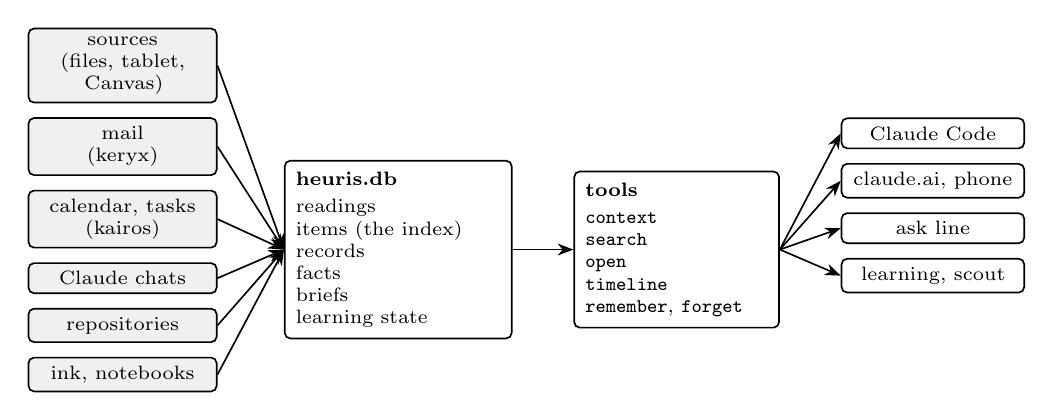
\begin{tikzpicture}[
  src/.style={draw,rounded corners=2pt,fill=black!6,align=center,inner sep=3pt,text width=6.2em,font=\scriptsize},
  db/.style={draw,rounded corners=2pt,align=left,inner sep=4pt,text width=7.4em,font=\scriptsize},
  use/.style={draw,rounded corners=2pt,align=center,inner sep=3pt,text width=6em,font=\scriptsize}]
\node[src] (lib) {sources\\(files, tablet, Canvas)};
\node[src,below=0.5em of lib] (mail) {mail\\(keryx)};
\node[src,below=0.5em of mail] (cal) {calendar, tasks\\(kairos)};
\node[src,below=0.5em of cal] (chat) {Claude chats};
\node[src,below=0.5em of chat] (repo) {repositories};
\node[src,below=0.5em of repo] (ink) {ink, notebooks};
\node[db,right=2.4em of cal,yshift=-1.1em] (h) {\textbf{heuris.db}\\[2pt]readings\\items (the index)\\records\\facts\\briefs\\learning state};
\node[db,right=2.2em of h,text width=6.6em] (t) {\textbf{tools}\\[2pt]\texttt{context}\\\texttt{search}\\\texttt{open}\\\texttt{timeline}\\\texttt{remember}, \texttt{forget}};
\node[use,right=2.2em of t,yshift=4.2em] (cc) {Claude Code};
\node[use,below=0.5em of cc] (ai) {claude.ai, phone};
\node[use,below=0.5em of ai] (ask) {ask line};
\node[use,below=0.5em of ask] (lrn) {learning, scout};
\foreach \n in {lib,mail,cal,chat,repo,ink} \draw[->] (\n.east) -- (h.west);
\draw[->] (h) -- (t);
\foreach \n in {cc,ai,ask,lrn} \draw[->] (t.east) -- (\n.west);
\end{tikzpicture}

\small Everything is indexed into one database; every caller reaches it through the same tools. Acting (scheduling, drafting) stays with kairos and keryx.
\end{center}

\Sec{C. How everything gets in}

Sized to what exists, measured 28 October. Indexing runs on the server's GPU (the nomic model the library already uses) and costs nothing; only the model steps spend credit.

{\small\renewcommand{\arraystretch}{1.2}
\begin{tabularx}{\linewidth}{@{}l >{\hsize=0.8\hsize}Y >{\hsize=1.2\hsize}Y@{}}
\toprule
Kind & Size now; per week & What is indexed, and the model step \\
\midrule
Mail & 7,271 messages, about 6.4M tokens; about 250 & Messages from a person, or that you replied to or starred, cleaned of quoted text and signatures. A changed thread gets a short summary (Haiku); threads from people also get fact extraction (Sonnet) \prop. \\
Calendar, tasks & about 380 series, 41 tasks & Title, attendees, notes. No model step; facts such as an interview date are read directly. Family included. \\
Claude chats & 241 laptop sessions, about 2.7M tokens; about 35 & Your turns as written; Claude's answers in chunks. A record per session at its end (Sonnet). Facts only through \texttt{remember}. \\
Repositories & 7 repositories; about 125 commits & READMEs, docs, decision logs. A record per batch of commits (Haiku). Code is not indexed: an agent reads it live when it needs it. \\
Sources & 277 documents, about 3M tokens; a few & Read as now, faithfully, maths and figures included. The model passes move to the API in one batched call per document. \\
Ink, notebooks & 752 marks; about 100 & Transcriptions as items, tied to page and passage (Slice 0.12's capture). \\
Year 1 and 2 & syllabi only & \you{28 Oct}{Dont want to ingest all of y1 and y2 notes, but their syllabi for context is good.} Each course becomes a ``studied'' fact. \\
\bottomrule
\end{tabularx}}

\medskip
\textbf{What is left out} \youx{28 Oct}: the OQTS-shared mailbox; mailing lists and automated mail: \you{28 Oct}{mail items should only be from useful things, I do not want it filing up with random rubbish and mailing lists}. One exception: mail from firms and recruiters is always kept, because offer letters often come from automated HR systems \prop. Also left out: the server's headless sessions (\texttt{-tmp}), which are locus's own jobs; indexing them would have locus read itself.

\textbf{Everything else}: \you{28 Oct}{everything in mail, not OQTS-shared, family calendar yes, that is useful context too.} Your Brevan Howard internship notes are on the tablet and come in with it; your Millennium spring week notes are lost \youx{28 Oct}.

\textbf{Never stale (R10).} Every brief and fact carries the date it was last checked, and a brief names any source it has not seen since then \prop.

\Sec{D. How it is found, and who can call it}

\Sub{The tools}
Any Claude can call these: Claude Code on either machine, claude.ai on the laptop or phone, and the locus ask line \agreed{28 Oct}.

\begin{tabularx}{\linewidth}{@{}l Y@{}}
\toprule
Tool & What it does \\
\midrule
\texttt{context} & the relevant briefs, current facts and today, optionally about one thing; the cheap first call \\
\texttt{search} & everything, by words and meaning, reranked, as dated snippets with pointers; filters for kind, area, thing, person and dates \\
\texttt{open} & the whole thing behind a pointer: a mail thread, the chat around a turn, a page of a source (as an image where it has maths), a notebook page \\
\texttt{timeline} & what happened to a thing or with a person, in order, across every kind, between two dates \\
\texttt{remember} & a fact, from a chat, with your approval \\
\texttt{forget} & a wrong fact retired, with your approval \\
\texttt{markups}, \texttt{to\_remarkable} & unchanged \\
\bottomrule
\end{tabularx}

\medskip
\textbf{Approval costs nothing to build.} \texttt{remember} and \texttt{forget} are left off the allow list, so each call shows the permission prompt with the exact fact and you answer with one key. claude.ai connectors ask the same way. Your global CLAUDE.md tells Claude to offer a \texttt{remember} straight after a message of yours that states a fact worth keeping, and to call \texttt{context()} whenever a question touches your life, projects, courses or applications \prop. The Home chat, which cannot show a prompt, asks with its own \texttt{y/n} line (B) \you{10 Nov}{does approve work in the chat feature in home}.

\Sub{Acting from anywhere}
You asked whether this means scheduling and drafting from anywhere: \you{28 Oct}{being able to say what emails are in my inbox right now that need responding and schedule drafts for them all.} Yes. heuris finds; the app that owns a thing acts. kairos's tools already let any Claude schedule, within kairos's risk rules. keryx gets a few tools of its own, in keryx's slice beside H1: list the threads that need a reply, read a thread, create a draft. It never sends; you send from Mail \prop. Nothing is done twice.

\Sub{Citing}
\you{28 Oct}{facts should be exactly recalled, but any sort of notes/ anything else that claude realistically would know anyways from training can just be referenced back to where it read it without the full quote. Just like a citation etc.} So:
\begin{itemize}
\item \textbf{Facts and decisions} are recalled exactly, with their source.
\item \textbf{Everything else} is cited like a reference, \textit{[B14 notes, p.~12]}, and the answering Claude explains around it and fills the gaps.
\end{itemize}
This changes CLAUDE.md invariant~1 for answers; it stays in force for everything stored. \you{28 Oct}{change to invariant 1 correct.}

\Sub{How each caller gets the tools}
\begin{itemize}
\item \textbf{Claude Code}: the one HTTP service (Slice 0.6) is registered once at user level, so every repository on either machine has it.
\item \textbf{claude.ai}, laptop and phone: the service is reachable over public HTTPS through Tailscale Funnel, with authentication. \you{28 Oct}{tailscale funnel fine, that is very safe.} Not yet checked: which authentication claude.ai's custom connectors accept. That is the first step of H1.
\item \textbf{The ask line}: the same tools, in a Sonnet tool loop on the server.
\end{itemize}

\Sub{Where heuris shows in the window}
No heuris pane \agreed{28 Oct}. The System view gets a heuris section: how fresh each source is, item counts, the credit pace. Facts are changed in chat or undone in the auto log.

\Sec{E. How it reasons, helps and teaches}

\Sub{Reasoning}
An answer is Claude deciding what to look up, not one fixed retrieval. The offers question pulls the facts about both offers, the offer threads, your earlier reasoning in chats, and the Jump outcome, then reasons over them. The library's search (hybrid, reranked) is the engine inside \texttt{search}. Hints and tips appear only where you look: \texttt{context()}, Home, the ask line. Nothing is pushed to you (R8). Explore and the scout become callers of the same tools \prop.

\Sub{The learning system: one shape}
\you{28 Oct}{I like the learning system - that taxonomy is good.} Every goal has five parts:
\begin{enumerate}
\item \textbf{A target}: an exam, an internship, an interview.
\item \textbf{A syllabus}, taken from a course's syllabus, or derived from a role, your CV, or a call's notes.
\item \textbf{Tracks}, each with a confidence level. Tracks are shared: probability practised for the exams also counts for Millennium.
\item \textbf{Sessions}, scheduled in kairos.
\item \textbf{Practice that is marked}, and the marks move the confidence levels.
\end{enumerate}
\textbf{One track can serve several targets} \you{10 Nov}{one learning track $\to$ multiple targets}. Your examples: C++ for oxdaq and quant work; the green book for Jump and HFT tests; linear algebra and statistics for both. A goal also carries the dates around its target, such as when applications open next year and the Millennium dates.

\textbf{A new topic} gets a structure of its own \you{10 Nov}{some sort of structure for learning new topics}: an initial scope of your ability, a skill tree built from it, then the practise, review and test cycle.

Goals are opt-in, never one per course \youx{Slice 1}. What differs between goals is only where the syllabus comes from and what practice looks like:

\begin{tabularx}{\linewidth}{@{}l Y Y@{}}
\toprule
& Exam revision & Millennium QD 2027 \\
\midrule
Syllabus from & the course syllabus first, slides and notes for detail & your QD call notes, the role, your CV \\
Practice & past papers & coding problems and small builds \\
\bottomrule
\end{tabularx}

\Sub{Revision}
How you revise now: you write full handwritten notes from slides, lecture notes and sheets, then cram past papers. \you{28 Oct}{the writing is the learning process and I learn while doing them, but I feel the time taken to learning ratio is skewed in the wrong direction.} You learn most from exam questions. The research on learning agrees: practice testing and spaced practice rank highest; rereading and summarising rank lowest.

\textbf{The course map} comes from the syllabus first: \you{28 Oct}{map of each course should primarily be derived from the syllabus, as that is what will be examined}. Slides and notes add the detail, and each past-paper question is placed against the topics it tests.

\noindent\begin{minipage}{\linewidth}
\textbf{The cycle for each module} \agreed{28 Oct}:
\begin{center}
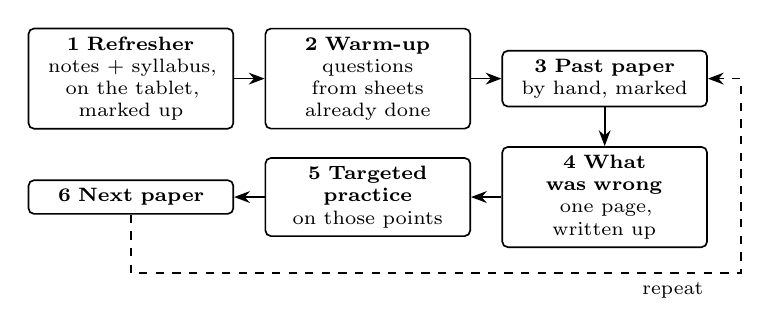
\begin{tikzpicture}[node distance=1.4em and 1.1em,
  st/.style={draw,rounded corners=2pt,align=center,inner sep=3pt,text width=6.8em,font=\scriptsize}]
\node[st] (r) {\textbf{1 Refresher}\\notes + syllabus, on the tablet, marked up};
\node[st,right=of r] (w) {\textbf{2 Warm-up}\\questions from sheets already done};
\node[st,right=of w] (p) {\textbf{3 Past paper}\\by hand, marked};
\node[st,below=of p] (x) {\textbf{4 What was wrong}\\one page, written up};
\node[st,left=of x] (t) {\textbf{5 Targeted practice}\\on those points};
\node[st,left=of t] (n) {\textbf{6 Next paper}};
\draw[->] (r) -- (w); \draw[->] (w) -- (p); \draw[->] (p) -- (x); \draw[->] (x) -- (t); \draw[->] (t) -- (n);
\coordinate (lo) at ($(x.south)+(0,-0.9em)$);
\coordinate (rt) at ($(x.east)+(1.2em,0)$);
\draw[->,dashed] (n.south) |- (lo) -- node[below,font=\scriptsize]{repeat} (lo -| rt) |- (p.east);
\end{tikzpicture}
\end{center}
\end{minipage}

\begin{itemize}
\item \textbf{For a new topic, a baseline quiz comes before the refresher}, so the gaps are known before anything is taught \you{10 Nov}{for new topic the refresher is preceded by a baseline quiz - so we know where the gaps are}.
\item \textbf{The refresher comes first} because \you{28 Oct}{jumping straight into questions I cannot do is demoralising.} It is built from your notes and the syllabus and pushed to the tablet. You mark it with what you had forgotten and what you do not know how to do: \you{28 Oct}{a great seed for where I stand}. Its readback sets each track's starting confidence.
\item \textbf{Notes come after attempts, not before.} You still write notes, since writing is how you learn, but one condensed page per topic, aimed at what you got wrong. heuris supplies the sources' essentials, so tired note-writing stops being transcription.
\item \textbf{Papers are marked} against the mark scheme where one exists; the marks move the topic's confidence.
\item \textbf{kairos schedules it}, mixing topics across blocks, weighted by weakness and by the exam date.
\end{itemize}
\textbf{When.} Revision happens in the vacations, with a real break after each term ends, Michaelmas included: \you{28 Oct}{the break is after any term finishes, so after MT as well.} Some in the winter vacation, so Easter carries less. None in Michaelmas or Hilary term: \you{28 Oct}{Term time is too busy for revision}. Trinity term, after lectures stop, is to be seen. Exams are in weeks 8 and 9 of Trinity \youx{28 Oct}.

\Sec{F. What it costs, and how the credit is guarded}

\Sub{Where model calls run}
Max 5x includes \$100 of API credit a month (verified on Anthropic's pages: Messages and Batch API, not Claude Code; it expires each cycle and does not roll over). \you{28 Oct}{I would put the bulk work on the api, and anything else if we are sure it will stay under the limit.} So every model call locus makes runs on the credit, through the Batch API wherever nobody is waiting, with prompt caching on repeated context. Your own chats stay on your subscription. Headless \texttt{claude -p} remains only as the fallback when the credit is spent. Running unattended jobs through an API key is also the route Anthropic's terms explicitly allow.

\Sub{Estimated monthly cost}
Every figure here is a \prop, to be replaced by the first month's measurement.

{\small
\begin{tabularx}{\linewidth}{@{}Y r@{}}
\toprule
Job (model) & per month \\
\midrule
Mail thread summaries (Haiku, batch) and facts (Sonnet, batch) & \$2 \\
Chat records (Sonnet, batch) & \$3 \\
Commit records (Haiku, batch) & under \$1 \\
Briefs rebuilt, about 200 times (Sonnet, batch, cached) & \$8 \\
Source ingest, model passes (Haiku, batch) & under \$1 \\
Ask-line answers, about 100 (Sonnet, cached) & \$10 \\
Refreshers, practice, marking, explainers (Sonnet; Opus for syllabi) & \$5--15 \\
\midrule
Total & \$30--40 \\
One-off backfill of all history (mail older than two years on Haiku only) & about \$15 \\
\bottomrule
\end{tabularx}}

\medskip
Prices used: Haiku 5.5 \$0.10 in and \$0.50 out per million tokens, Sonnet 5.5 \$2 and \$10, halved in batch. These are estimates; the first month is measured and this table replaced with what happened.

\Sub{The guard}
\begin{itemize}
\item A credit ledger allows, each day, the credit remaining divided by the days remaining \prop.
\item Answers you are waiting for have a 30\% reserve; bulk work waits for the next cycle rather than overspend \prop.
\item If the credit is ever spent, answers fall back to the subscription; nothing is charged, since an empty credit only refuses requests.
\item In the last days of a cycle, what is left goes to Explore and the scout \youx{28 Oct}.
\item The budget bar on Home becomes ``credit \$x of \$100, on pace for \$y'' beside your 5-hour window; you accepted that it changes form \youx{28 Oct}.
\end{itemize}

\Sec{G. What happens to the old engine}

\begin{tabularx}{\linewidth}{@{}l Y@{}}
\toprule
Keep & reading PDFs with maths and figures; chunking; nomic vectors; full-text search; the reranker; ingest by content hash and the one-ingest lock; ink capture; tablet push; LaTeX; \texttt{gates} and \texttt{mcp-log}; the evaluation harness, rebuilt around the test set (J) \\
Change & \texttt{retrieve} becomes \texttt{search}, with filters; model passes move to the API in batches, one call per document; notebook and margin transcriptions become items; the MCP becomes the HTTP service with the tools in D; \texttt{locus.db} migrates into \texttt{heuris.db} \\
Drop & propositions, entities, aliases, related, threads, connect, structure, evolve, critique and synthesise, the old discover, decide, the Obsidian export, and their tables \prop \\
\bottomrule
\end{tabularx}

\medskip
\textbf{Is this the best engine for the goals?} \you{10 Nov}{do you think this leaves us with the best possible new engine?} Yes. Two things make it better than the old one rather than only cheaper. The model passes leave the local 8B model, which was the ceiling on every summary and extraction (CLAUDE.md \S14, \S11.B). And Claude reasoning with tools replaces one fixed retrieval, which is what the linking failures needed. \textbf{What is kept after the migration} is what cannot be regenerated: the readings of every source (the expensive maths reading), your ink and its transcriptions, the content hashes, the gate and call logs. Everything derived is rebuilt from those, so nothing you wrote is lost when \texttt{locus.db} is retired.

\textbf{One measurement before dropping.} Propositions are a search arm today. The retrieval evaluation runs with and without them on the test set; they go if answers do not get worse \prop. Everything else on the drop list is either unused or already off.

\Sec{H. Changes to the plan and to CLAUDE.md}
\begin{itemize}
\item \textbf{Invariant 1} (grounded or silent) holds for everything stored; answers cite like references and explain around them (D).
\item \textbf{Slice 0.13} moved every model call to the subscription; locus's calls now run on the API credit, with the subscription as fallback (F). \texttt{agent/claude.py} stays the one runner, with two backends.
\item \textbf{The notes repository} (plan C.9) becomes \textbf{files}, and transcriptions leave it (B).
\item \textbf{Area briefs} (plan C.13) become heuris's briefs, one per thing and one about you, built from facts.
\item \textbf{Search over everything} moves from Slice 7 to H1.
\item \textbf{The learning system} moves up and takes in revision (E); interview preparation is one kind of goal, as before.
\item \textbf{Two databases become one} (B).
\end{itemize}

\Sec{I. Build order}
\you{28 Oct}{I just want to build the best system possible however we can, and if this order gets us there then that is good with me.} Reordered on 10 November to your 9 November priorities: Home live, then mail that derives truth, then the career plan; Home live needs nothing from heuris, so it comes first and is in use while the rest is built \youx{10 Nov, agreed}.

{\small\renewcommand{\arraystretch}{1.15}
\begin{tabularx}{\linewidth}{@{}l >{\hsize=1.3\hsize}Y >{\hsize=0.7\hsize}Y@{}}
\toprule
Slice & What & Done when \\
\midrule
4 & \textbf{Home live}: your projects from the registry, git, kairos and tmux, built now without heuris \you{9 Nov}{wished home page project view was live}. & Home replaces checking things by hand. \\
0 & \textbf{Plumbing, finishing.} The 0.6 HTTP service becomes heuris's home. Budget logging (0.7) grows into the credit ledger and the API backend. & As in the Slice 0 spec, plus one batched job paid from the credit. \\
H1 & \textbf{The index and the tools.} \texttt{heuris.db}; items from every source with their filters; \texttt{context}, \texttt{search}, \texttt{open}, \texttt{timeline}; registered at user level on both machines; the claude.ai check. keryx's tools beside it. The Home chat gets search. & Every test question the data can answer is answered well from a fresh chat with no pasted context. \\
H2 & \textbf{What is true now.} Records, facts, briefs, \texttt{remember} and \texttt{forget} (with the Home chat's \texttt{y/n}), syllabi. Facts from mail are your ``mail that derives truth'': application status, deadlines, cleanup; they feed Home's careers panel and the career plan. & The offers, mail and Jump-feedback questions come back with the right current state; a CV description of nabla is accurate. \\
L & \textbf{Learning and revision} (was Slice 6). Goals, syllabi, shared tracks; the module cycle and the new-topic structure; refreshers on the tablet; marked practice. In time for the winter vacation. & One real goal and one module run through it. \\
\midrule
\multicolumn{3}{@{}l}{\textit{Set aside on 9 November, back only when you ask:} Project view live (3); dossiers and the ink gate (2);}\\
\multicolumn{3}{@{}l}{\textit{linking, Explore and the scout (5); canvas and charts (7).}}\\
\bottomrule
\end{tabularx}}

\clearpage
\Sec{J. The test set}
The foundational test of heuris: questions you would actually ask, so the system is not built only on what was useful in the last few weeks. You wrote the first nine; the rest were proposed on 28 October and you approved them: \you{28 Oct}{so basically all of these are actually good questions that I would ask}. Brackets mark a placeholder to fill in. Each question gets a line from you on what a good answer contains, and is scored on three things: the right current state, the right sources found, and nothing invented.

\Sub{Yours}
{\small\begin{enumerate}[label=Y\arabic*.]
\item I have a Millennium Quantitative Developer offer, and also a Brevan Howard EM Rates Trading offer for summer internship 2027. Help me reason through why I should pick each one.
\item What did I write on the Millennium role preference form they sent after the spring week? From that, why do you think they put me on the quant dev track rather than QR?
\item Look through the Brevan Howard notes I made over the internship and draw on other projects and notes to theorise about how to improve nabla.
\item Use the problem sheet and notes on image processing from my recent lectures to explain how CNNs work, with an example of their use in quantitative finance.
\item Across my quant finance projects, why have we never really been able to approach deep learning, and where could my projects (quant finance or not) benefit from it?
\item Could any of my projects or ideas be built out or refactored into a startup over the next two years, while I do not have to apply for internships?
\item Have I missed any emails I need to reply to? What is the current state of Brevan Howard's offer, and what would it mean to renege on it?
\item Create a learning track for learning in depth every concept in my CV, with coding in the curriculum, then plan 2 hours a week for it.
\item Look at my rough notes from the Jump Trading feedback call, map out my weaknesses and plan a curriculum to be better prepared next year when they have told me to reapply. (It should know next year comes after the Millennium internship.)
\end{enumerate}}

\Sub{Facts and current state}
{\small\begin{enumerate}[label=\arabic*.]
\item What deadlines or interviews do I have coming up in careers, and what do I still owe anyone?
\item When did I last hear from [BH recruiter], and what did I last tell them?
\item Did I agree to anything in an email that is not in my calendar yet?
\item When did I last work on quast, and what was I in the middle of?
\item Why did nabla drop the momentum family?
\item Which version of my CV went to G-Research?
\end{enumerate}}

\Sub{Linking}
{\small\begin{enumerate}[label=\arabic*.,start=7]
\item Which lectures this term bear on quast, specifically?
\item Is there anything in B15 Control that nabla's regime work could use?
\item Have I read or noted anything that bears on tanker-flow's nowcast?
\item Which of my margin notes on papers connect to a project I am working on now?
\item Have I solved a problem like this one before in another project? (an error pasted, or a bug described)
\item From my BH internship notes, which ideas could apply to quast or OQTS, not only to nabla?
\item Which papers I have read, and my notes on them, hold ideas I could use in my projects, or for a new one? \youx{28 Oct, added}
\end{enumerate}}

\Sub{Describing my own work}
{\small\begin{enumerate}[label=\arabic*.,start=14]
\item Write three CV bullets for nabla with the real numbers.
\item What is quast's best result now, and where did it start?
\item What changed in locus this week?
\item Explain oxdaq to an interviewer in two minutes, accurately.
\end{enumerate}}

\Sub{Exact source content}
{\small\begin{enumerate}[label=\arabic*.,start=18]
\item State [theorem or definition] exactly as it is in [B15 lecture N].
\item Show me the figure in the B14 slides that explains convolution.
\item What did I write in the margin of \textit{Advanced Portfolio Management} about [topic]?
\item Find the page of my B14 notes where I worked through 2D Fourier transforms, and open it there.
\end{enumerate}}

\Sub{Mail and acting}
{\small\begin{enumerate}[label=\arabic*.,start=22]
\item What emails need a reply? Draft replies for them all.
\item Schedule the meeting the 3YP group proposed in their last email.
\item What are the start date and terms in my Millennium offer?
\item Who has not answered an email of mine that needed an answer?
\item I am meeting [person] tomorrow. Brief me on everything between us.
\end{enumerate}}

\Sub{Learning and revision}
{\small\begin{enumerate}[label=\arabic*.,start=27]
\item Which topics in the B15 syllabus have lectures covered so far, and which am I weakest at?
\item Give me a 30-minute refresher on [topic] from my notes before I attempt the past paper.
\item Mark my answers to [B14 paper, question] that I wrote on the tablet.
\item Plan my winter vacation: revision for the B courses alongside Millennium preparation.
\item What did I study in years 1 and 2 that is relevant to stochastic calculus?
\item Which past-paper question types do I keep getting wrong?
\end{enumerate}}

\Sub{Careers}
{\small\begin{enumerate}[label=\arabic*.,start=33]
\item Across all my interviews, which question types keep coming up?
\item Write a cover-letter paragraph for [firm] using my real projects.
\item I've been accepted to the G-Research x Oxford Edge AI/ML Quant Challenges. Which projects should I aim for, given that I want to work close to systematic at Millennium this summer (alt data or rates), then stay on or go to a graduate role at a systematic or HFT firm (Tower, Jump, G-Research, HRT, QRT)? \you{31 Oct}{I would have hopefully discussed my preferences in a claude.ai chat and they would have been saved in a remember ask.} A good answer uses the acceptance mail and its brief, the Millennium offer, my approved preferences and my real projects and courses.
\end{enumerate}}

\Sub{Planning and advice} {\small\youx{10 Nov, added: ``want it to include advice/help with planning time \ldots{} many different projects/things to do at the moment; add learning examples to test set''}}
{\small\begin{enumerate}[label=P\arabic*.]
\item I have many projects and things to do at the moment. Which deserve my time this week, and how should I split it?
\item Plan this week around my lectures, the projects that are live and what is due.
\item Build me a learning track for C++ aimed at oxdaq and quant developer work, and say how it shares ground with Millennium preparation.
\item Start me on the green book for Jump and HFT tests: what is my baseline, and what comes first?
\item Which linear algebra and statistics would serve both my B courses and Millennium, and where am I weakest?
\end{enumerate}}

\Sub{Patterns over time}
{\small\begin{enumerate}[label=\arabic*.,start=36]
\item How much time did I spend on each project last month, against what I planned?
\item What have I been putting off for more than two weeks?
\item What did I mainly do in September?
\item What project ideas have I had over the past year?
\item On the phone, in claude.ai: what is on tomorrow, and is there anything I need to prepare?
\end{enumerate}}

\Sub{Personal}
{\small\begin{enumerate}[label=\arabic*.,start=41]
\item What is on the family calendar over Christmas, and does it clash with anything of mine?
\end{enumerate}}

\Sub{Integrity: answers that must not go wrong}
{\small\begin{enumerate}[label=\arabic*.,start=42]
\item After a chat where I say ``suppose I took the Jump offer'': did I get a Jump offer? It must say no.
\item Am I still waiting on Jump? It must say no, from the newer fact.
\item Find the Brevan Howard offer email, which comes from an automated HR system. The mail filter must not have dropped it.
\item What did I write in my Millennium spring week notes? It must say they do not exist, not invent them.
\item What did Sam say? With two Sams, it must ask which, or name both.
\item Anything from the OQTS-shared mailbox. It must never appear.
\item Explain how quast's barrier tuning works. Every claim must match the repository.
\end{enumerate}}

\noindent{\small Personal and Integrity were not named one by one in your reply; they are taken as approved from ``basically all of these''. Strike any you do not want.}

\Sec{K. Still open}
\begin{itemize}
\item \textbf{First step of H1:} which authentication claude.ai's custom connectors accept, and so how the Funnel is protected.
\item \textbf{Decided in H1 by looking at real data, not guessed now} \you{10 Nov}{explain better what you mean}: which fields each indexed item carries; how quoted replies and signatures are stripped from a mail thread; what counts as mail ``from a person'' rather than automated; whether the tools are registered at user level on the server as well as the laptop. Each is quicker and more reliable to settle with real items in front of us.
\item \textbf{Decided in H2:} what a brief looks like and how long it is; how facts are named so a newer one finds the one it replaces; whether chats on claude.ai are brought in (they live only in Anthropic's export).
\item \textbf{Slice 0, separately:} capture logged ``unmapped'' in 2,724 of 2,742 runs. That has the shape of CLAUDE.md \S3's silent failure and is checked in Slice 0.12 whatever is decided here.
\item \textbf{The dossier} is set aside with the Project view \you{10 Nov}{retired project section for now}.
\item \textbf{Anything else:} \you{10 Nov}{general advice help etc ideating/ thinking about things but I think this is covered}. It is: that is the Home chat and any Claude with the tools.
\end{itemize}

\end{document}
